\chapter{Tổ hợp}

\index{combinatorics}

\key{Tổ hợp (Combinatorics)} nghiên cứu các phương pháp đếm
các kết hợp của các đối tượng.
Thông thường, mục tiêu là tìm ra một cách để
đếm các kết hợp một cách hiệu quả
mà không cần tạo ra từng kết hợp riêng lẻ.

Ví dụ, hãy xem xét bài toán
đếm số cách để
biểu diễn một số nguyên $n$ dưới dạng tổng của các số nguyên dương.
Ví dụ, có 8 cách biểu diễn
cho số 4:
\begin{multicols}{2}
\begin{itemize}
\item $1+1+1+1$
\item $1+1+2$
\item $1+2+1$
\item $2+1+1$
\item $2+2$
\item $3+1$
\item $1+3$
\item $4$
\end{itemize}
\end{multicols}

Một bài toán tổ hợp thường có thể được giải quyết
bằng một hàm đệ quy.
Trong bài toán này, chúng ta có thể định nghĩa một hàm $f(n)$
cho ra số cách biểu diễn của $n$.
Ví dụ, $f(4)=8$ theo ví dụ trên.
Các giá trị của hàm
có thể được tính đệ quy như sau:
\begin{equation*}
    f(n) = \begin{cases}
               1               & n = 0\\
               f(0)+f(1)+\cdots+f(n-1) & n > 0\\
           \end{cases}
\end{equation*}
Trường hợp cơ sở là $f(0)=1$,
bởi vì tổng rỗng biểu diễn số 0.
Sau đó, nếu $n>0$, chúng ta xem xét tất cả các cách để
chọn số đầu tiên của tổng.
Nếu số đầu tiên là $k$,
có $f(n-k)$ cách biểu diễn
cho phần còn lại của tổng.
Do đó, chúng ta tính tổng của tất cả các giá trị
có dạng $f(n-k)$ trong đó $k<n$.

Các giá trị đầu tiên của hàm là:
\[
\begin{array}{lcl}
f(0) & = & 1 \\
f(1) & = & 1 \\
f(2) & = & 2 \\
f(3) & = & 4 \\
f(4) & = & 8 \\
\end{array}
\]

Đôi khi, một công thức đệ quy có thể được thay thế
bằng một công thức dạng đóng.
Trong bài toán này,
\[
f(n)=2^{n-1},
\]
dựa trên thực tế là có $n-1$
vị trí có thể cho các dấu +- trong tổng
và chúng ta có thể chọn bất kỳ tập hợp con nào trong số chúng.

\section{Tổ hợp chập (Binomial coefficients)}

\index{binomial coefficient}

\key{Tổ hợp chập (Binomial coefficient)} ${n \choose k}$
bằng số cách chúng ta có thể chọn một tập hợp con
gồm $k$ phần tử từ một tập hợp gồm $n$ phần tử.
Ví dụ, ${5 \choose 3}=10$,
bởi vì tập hợp $\{1,2,3,4,5\}$
có 10 tập hợp con gồm 3 phần tử:
\[ \{1,2,3\}, \{1,2,4\}, \{1,2,5\}, \{1,3,4\}, \{1,3,5\}, 
\{1,4,5\}, \{2,3,4\}, \{2,3,5\}, \{2,4,5\}, \{3,4,5\} \]

\subsubsection{Công thức 1}

Tổ hợp chập có thể được
tính đệ quy như sau:

\[
{n \choose k}  =  {n-1 \choose k-1} + {n-1 \choose k}
\]

Ý tưởng là cố định một phần tử $x$ trong tập hợp.
Nếu $x$ được bao gồm trong tập hợp con,
chúng ta phải chọn $k-1$
phần tử từ $n-1$ phần tử,
và nếu $x$ không được bao gồm trong tập hợp con,
chúng ta phải chọn $k$ phần tử từ $n-1$ phần tử.

Các trường hợp cơ sở cho đệ quy là
\[
{n \choose 0}  =  {n \choose n} = 1,
\]
bởi vì luôn có chính xác
một cách để xây dựng một tập hợp con rỗng
và một tập hợp con chứa tất cả các phần tử.

\subsubsection{Công thức 2}

Một cách khác để tính tổ hợp chập như sau:
\[
{n \choose k}  =  \frac{n!}{k!(n-k)!}.
\]

Có $n!$ hoán vị của $n$ phần tử.
Chúng ta duyệt qua tất cả các hoán vị và luôn
bao gồm $k$ phần tử đầu tiên của hoán vị
trong tập hợp con.
Vì thứ tự của các phần tử trong tập hợp con
và bên ngoài tập hợp con không quan trọng,
kết quả được chia cho $k!$ và $(n-k)!$

\subsubsection{Các thuộc tính}

Đối với tổ hợp chập,
\[
{n \choose k}  =  {n \choose n-k},
\]
bởi vì thực tế chúng ta chia một tập hợp gồm $n$ phần tử thành
hai tập hợp con: tập hợp thứ nhất chứa $k$ phần tử
và tập hợp thứ hai chứa $n-k$ phần tử.

Tổng của các tổ hợp chập là
\[
{n \choose 0}+{n \choose 1}+{n \choose 2}+\ldots+{n \choose n}=2^n.
\]

Lý do cho tên "tổ hợp chập"
có thể được nhìn thấy khi nhị thức $(a+b)$ được nâng lên
lũy thừa thứ $n$:

\[ (a+b)^n =
{n \choose 0} a^n b^0 + 
{n \choose 1} a^{n-1} b^1 +
\ldots + 
{n \choose n-1} a^1 b^{n-1} +
{n \choose n} a^0 b^n. \]

\index{Pascal's triangle}

Tổ hợp chập cũng xuất hiện trong
\key{tam giác Pascal (Pascal's triangle)}
trong đó mỗi giá trị bằng tổng của hai
giá trị phía trên:
\begin{center}
\begin{tikzpicture}{0.9}
\node at (0,0) {1};
\node at (-0.5,-0.5) {1};
\node at (0.5,-0.5) {1};
\node at (-1,-1) {1};
\node at (0,-1) {2};
\node at (1,-1) {1};
\node at (-1.5,-1.5) {1};
\node at (-0.5,-1.5) {3};
\node at (0.5,-1.5) {3};
\node at (1.5,-1.5) {1};
\node at (-2,-2) {1};
\node at (-1,-2) {4};
\node at (0,-2) {6};
\node at (1,-2) {4};
\node at (2,-2) {1};
\node at (-2,-2.5) {$\ldots$};
\node at (-1,-2.5) {$\ldots$};
\node at (0,-2.5) {$\ldots$};
\node at (1,-2.5) {$\ldots$};
\node at (2,-2.5) {$\ldots$};
\end{tikzpicture}
\end{center}

\subsubsection{Hộp và bóng}

"Hộp và bóng" là một mô hình hữu ích,
trong đó chúng ta đếm số cách để
đặt $k$ quả bóng vào $n$ hộp.
Hãy xem xét ba kịch bản:

\textit{Kịch bản 1}: Mỗi hộp có thể chứa
nhiều nhất một quả bóng.
Ví dụ, khi $n=5$ và $k=2$,
có 10 giải pháp:

\begin{center}
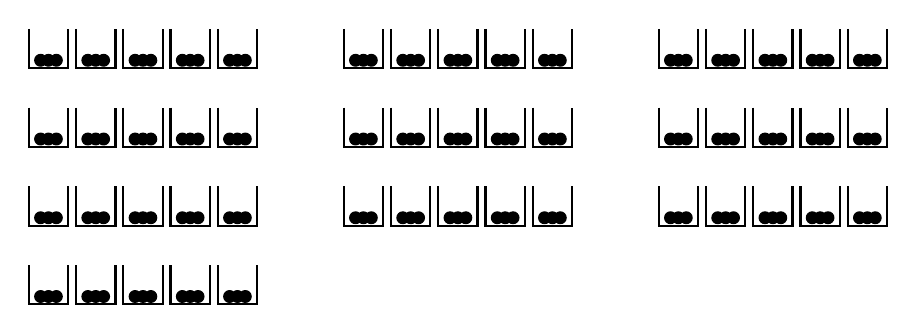
\begin{tikzpicture}[scale=0.5]
\newcommand\lax[3]{
\path[draw,thick,-] (#1-0.5,#2+0.5) -- (#1-0.5,#2-0.5) --
                    (#1+0.5,#2-0.5) -- (#1+0.5,#2+0.5);
\ifthenelse{\equal{#3}{1}}{\draw[fill=black] (#1,#2-0.3) circle (0.15);}{}
\ifthenelse{\equal{#3}{2}}{\draw[fill=black] (#1-0.2,#2-0.3) circle (0.15);}{}
\ifthenelse{\equal{#3}{2}}{\draw[fill=black] (#1+0.2,#2-0.3) circle (0.15);}{}
}
\newcommand\laa[7]{
    \lax{#1}{#2}{#3}
    \lax{#1+1.2}{#2}{#4}
    \lax{#1+2.4}{#2}{#5}
    \lax{#1+3.6}{#2}{#6}
    \lax{#1+4.8}{#2}{#7}
}

\laa{0}{0}{1}{1}{0}{0}{0}
\laa{0}{-2}{1}{0}{1}{0}{0}
\laa{0}{-4}{1}{0}{0}{1}{0}
\laa{0}{-6}{1}{0}{0}{0}{1}
\laa{8}{0}{0}{1}{1}{0}{0}
\laa{8}{-2}{0}{1}{0}{1}{0}
\laa{8}{-4}{0}{1}{0}{0}{1}
\laa{16}{0}{0}{0}{1}{1}{0}
\laa{16}{-2}{0}{0}{1}{0}{1}
\laa{16}{-4}{0}{0}{0}{1}{1}

\end{tikzpicture}
\end{center}

Trong kịch bản này, câu trả lời trực tiếp là
tổ hợp chập ${n \choose k}$.

\textit{Kịch bản 2}: Một hộp có thể chứa nhiều quả bóng.
Ví dụ, khi $n=5$ và $k=2$,
có 15 giải pháp:

\begin{center}
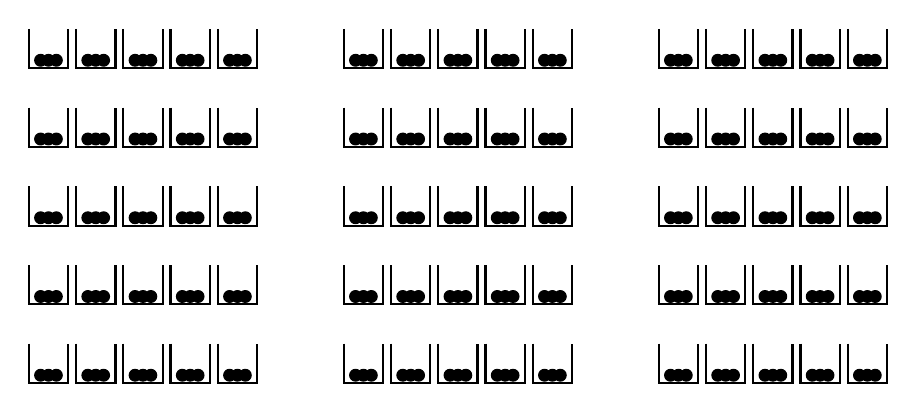
\begin{tikzpicture}[scale=0.5]
\newcommand\lax[3]{
\path[draw,thick,-] (#1-0.5,#2+0.5) -- (#1-0.5,#2-0.5) --
                    (#1+0.5,#2-0.5) -- (#1+0.5,#2+0.5);
\ifthenelse{\equal{#3}{1}}{\draw[fill=black] (#1,#2-0.3) circle (0.15);}{}
\ifthenelse{\equal{#3}{2}}{\draw[fill=black] (#1-0.2,#2-0.3) circle (0.15);}{}
\ifthenelse{\equal{#3}{2}}{\draw[fill=black] (#1+0.2,#2-0.3) circle (0.15);}{}
}
\newcommand\laa[7]{
    \lax{#1}{#2}{#3}
    \lax{#1+1.2}{#2}{#4}
    \lax{#1+2.4}{#2}{#5}
    \lax{#1+3.6}{#2}{#6}
    \lax{#1+4.8}{#2}{#7}
}

\laa{0}{0}{2}{0}{0}{0}{0}
\laa{0}{-2}{1}{1}{0}{0}{0}
\laa{0}{-4}{1}{0}{1}{0}{0}
\laa{0}{-6}{1}{0}{0}{1}{0}
\laa{0}{-8}{1}{0}{0}{0}{1}
\laa{8}{0}{0}{2}{0}{0}{0}
\laa{8}{-2}{0}{1}{1}{0}{0}
\laa{8}{-4}{0}{1}{0}{1}{0}
\laa{8}{-6}{0}{1}{0}{0}{1}
\laa{8}{-8}{0}{0}{2}{0}{0}
\laa{16}{0}{0}{0}{1}{1}{0}
\laa{16}{-2}{0}{0}{1}{0}{1}
\laa{16}{-4}{0}{0}{0}{2}{0}
\laa{16}{-6}{0}{0}{0}{1}{1}
\laa{16}{-8}{0}{0}{0}{0}{2}

\end{tikzpicture}
\end{center}

Quá trình đặt các quả bóng vào các hộp
có thể được biểu diễn dưới dạng một chuỗi
bao gồm các ký hiệu
"o" và "$\rightarrow$".
Ban đầu, giả sử rằng chúng ta đang đứng ở hộp ngoài cùng bên trái.
Ký hiệu "o" có nghĩa là chúng ta đặt một quả bóng
vào hộp hiện tại, và ký hiệu
"$\rightarrow$" có nghĩa là chúng ta di chuyển đến
hộp tiếp theo bên phải.

Sử dụng ký hiệu này, mỗi giải pháp là một chuỗi
chứa $k$ lần ký hiệu "o" và
$n-1$ lần ký hiệu "$\rightarrow$".
Ví dụ, giải pháp trên cùng bên phải
trong hình trên tương ứng với chuỗi
"$\rightarrow$ $\rightarrow$ o $\rightarrow$ o $\rightarrow$".
Do đó, số lượng các giải pháp là
${k+n-1 \choose k}$.

\textit{Kịch bản 3}: Mỗi hộp có thể chứa nhiều nhất một quả bóng,
và ngoài ra, không có hai hộp liền kề nào có thể cùng chứa một quả bóng.
Ví dụ, khi $n=5$ và $k=2$,
có 6 giải pháp:


\begin{center}
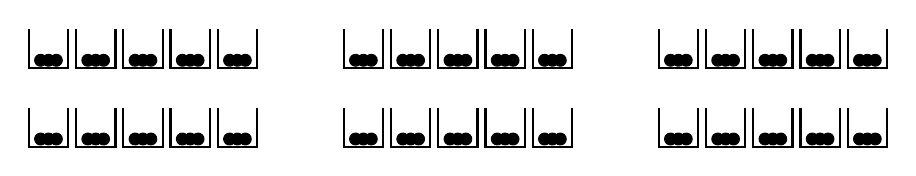
\begin{tikzpicture}[scale=0.5]
\newcommand\lax[3]{
\path[draw,thick,-] (#1-0.5,#2+0.5) -- (#1-0.5,#2-0.5) --
                    (#1+0.5,#2-0.5) -- (#1+0.5,#2+0.5);
\ifthenelse{\equal{#3}{1}}{\draw[fill=black] (#1,#2-0.3) circle (0.15);}{}
\ifthenelse{\equal{#3}{2}}{\draw[fill=black] (#1-0.2,#2-0.3) circle (0.15);}{}
\ifthenelse{\equal{#3}{2}}{\draw[fill=black] (#1+0.2,#2-0.3) circle (0.15);}{}
}
\newcommand\laa[7]{
    \lax{#1}{#2}{#3}
    \lax{#1+1.2}{#2}{#4}
    \lax{#1+2.4}{#2}{#5}
    \lax{#1+3.6}{#2}{#6}
    \lax{#1+4.8}{#2}{#7}
}

\laa{0}{0}{1}{0}{1}{0}{0}
\laa{0}{-2}{1}{0}{0}{1}{0}
\laa{8}{0}{1}{0}{0}{0}{1}
\laa{8}{-2}{0}{1}{0}{1}{0}
\laa{16}{0}{0}{1}{0}{0}{1}
\laa{16}{-2}{0}{0}{1}{0}{1}
\end{tikzpicture}
\end{center}

Trong kịch bản này, chúng ta có thể giả sử rằng
$k$ quả bóng ban đầu được đặt trong các hộp
và có một hộp trống giữa mỗi
hai hộp liền kề.
Nhiệm vụ còn lại là chọn các
vị trí cho các hộp trống còn lại.
Có $n-2k+1$ hộp như vậy và
$k+1$ vị trí cho chúng.
Do đó, sử dụng công thức của kịch bản 2,
số lượng các giải pháp là
${n-k+1 \choose n-2k+1}$.

\subsubsection{Hệ số đa thức}

\index{multinomial coefficient}

\key{Hệ số đa thức (multinomial coefficient)}
\[ {n \choose k_1,k_2,\ldots,k_m} = \frac{n!}{k_1! k_2! \cdots k_m!}, \]
bằng số cách
chúng ta có thể chia $n$ phần tử thành các tập hợp con
có kích thước $k_1,k_2,\ldots,k_m$,
trong đó $k_1+k_2+\cdots+k_m=n$.
Hệ số đa thức có thể được coi là một
sự tổng quát hóa của tổ hợp chập;
nếu $m=2$, công thức trên
tương ứng với công thức tổ hợp chập.

\section{Số Catalan}

\index{Catalan number}

\key{Số Catalan (Catalan number)}
$C_n$ bằng
số lượng các biểu thức
ngoặc hợp lệ bao gồm
$n$ dấu ngoặc trái và $n$ dấu ngoặc phải.

Ví dụ, $C_3=5$, bởi vì
chúng ta có thể xây dựng các biểu thức ngoặc
sau đây bằng cách sử dụng ba
dấu ngoặc trái và phải:

\begin{itemize}[noitemsep]
\item \texttt{()()()}
\item \texttt{(())()}
\item \texttt{()(())}
\item \texttt{((()))}
\item \texttt{(()())}
\end{itemize}

\subsubsection{Biểu thức ngoặc}

\index{parenthesis expression}

Chính xác thì \emph{biểu thức ngoặc hợp lệ} là gì?
Các quy tắc sau đây định nghĩa chính xác tất cả
các biểu thức ngoặc hợp lệ:

\begin{itemize}
\item Một biểu thức ngoặc rỗng là hợp lệ.
\item Nếu một biểu thức $A$ là hợp lệ,
thì biểu thức
\texttt{(}$A$\texttt{)} cũng là hợp lệ.
\item Nếu các biểu thức $A$ và $B$ là hợp lệ,
thì biểu thức $AB$ cũng là hợp lệ.
\end{itemize}

Một cách khác để mô tả các
biểu thức ngoặc hợp lệ là nếu
chúng ta chọn bất kỳ tiền tố nào của một biểu thức như vậy,
nó phải chứa ít nhất số dấu ngoặc trái
bằng số dấu ngoặc phải.
Ngoài ra, biểu thức hoàn chỉnh phải
chứa một số lượng bằng nhau các dấu ngoặc trái và phải.

\subsubsection{Công thức 1}

Các số Catalan có thể được tính bằng công thức
\[ C_n = \sum_{i=0}^{n-1} C_{i} C_{n-i-1}.\]

Tổng duyệt qua các cách để chia
biểu thức thành hai phần
sao cho cả hai phần đều là các biểu thức
hợp lệ và phần đầu tiên càng ngắn càng tốt
nhưng không rỗng.
Với bất kỳ $i$ nào, phần đầu tiên chứa $i+1$ cặp
dấu ngoặc và số lượng các biểu thức
là tích của các giá trị sau:

\begin{itemize}
\item $C_{i}$: số cách để xây dựng một biểu thức
sử dụng các dấu ngoặc của phần đầu tiên,
không tính các dấu ngoặc ngoài cùng
\item $C_{n-i-1}$: số cách để xây dựng một
biểu thức sử dụng các dấu ngoặc của phần thứ hai
\end{itemize}

Trường hợp cơ sở là $C_0=1$,
bởi vì chúng ta có thể xây dựng một biểu thức ngoặc
rỗng bằng cách sử dụng không cặp dấu ngoặc.

\subsubsection{Công thức 2}

Các số Catalan cũng có thể được tính
bằng tổ hợp chập:
\[ C_n = \frac{1}{n+1} {2n \choose n}\]
Công thức có thể được giải thích như sau:

Có tổng cộng ${2n \choose n}$ cách
để xây dựng một biểu thức ngoặc (không nhất thiết phải hợp lệ)
chứa $n$ dấu ngoặc trái
và $n$ dấu ngoặc phải.
Chúng ta hãy tính số lượng các
biểu thức như vậy \emph{không} hợp lệ.

Nếu một biểu thức ngoặc không hợp lệ,
nó phải chứa một tiền tố trong đó
số lượng dấu ngoặc phải vượt quá
số lượng dấu ngoặc trái.
Ý tưởng là đảo ngược mỗi dấu ngoặc
thuộc về một tiền tố như vậy.
Ví dụ, biểu thức
\texttt{())()(} chứa một tiền tố \texttt{())},
và sau khi đảo ngược tiền tố,
biểu thức trở thành \texttt{)((()(}.

Biểu thức kết quả bao gồm $n+1$
dấu ngoặc trái và $n-1$ dấu ngoặc phải.
Số lượng các biểu thức như vậy là ${2n \choose n+1}$,
bằng số lượng các biểu thức
ngoặc không hợp lệ.
Do đó, số lượng các biểu thức ngoặc
hợp lệ có thể được tính bằng công thức
\[{2n \choose n}-{2n \choose n+1} = {2n \choose n} - \frac{n}{n+1} {2n \choose n} = \frac{1}{n+1} {2n \choose n}.\]

\subsubsection{Đếm cây}

Các số Catalan cũng liên quan đến cây:

\begin{itemize}
\item có $C_n$ cây nhị phân gồm $n$ nút
\item có $C_{n-1}$ cây có gốc gồm $n$ nút
\end{itemize}
\noindent
Ví dụ, với $C_3=5$, các cây nhị phân là

\begin{center}
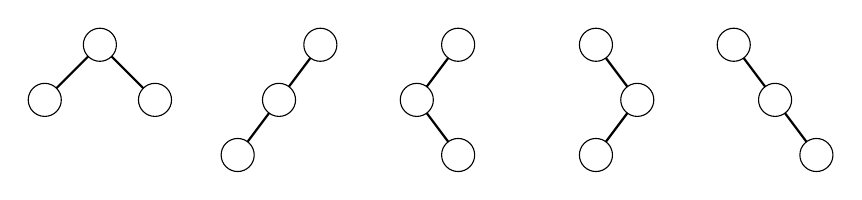
\begin{tikzpicture}[scale=0.7]
\path[draw,thick,-] (0,0) -- (-1,-1);
\path[draw,thick,-] (0,0) -- (1,-1);
\draw[fill=white] (0,0) circle (0.3);
\draw[fill=white] (-1,-1) circle (0.3);
\draw[fill=white] (1,-1) circle (0.3);

\path[draw,thick,-] (4,0) -- (4-0.75,-1) -- (4-1.5,-2);
\draw[fill=white] (4,0) circle (0.3);
\draw[fill=white] (4-0.75,-1) circle (0.3);
\draw[fill=white] (4-1.5,-2) circle (0.3);

\path[draw,thick,-] (6.5,0) -- (6.5-0.75,-1) -- (6.5-0,-2);
\draw[fill=white] (6.5,0) circle (0.3);
\draw[fill=white] (6.5-0.75,-1) circle (0.3);
\draw[fill=white] (6.5-0,-2) circle (0.3);

\path[draw,thick,-] (9,0) -- (9+0.75,-1) -- (9-0,-2);
\draw[fill=white] (9,0) circle (0.3);
\draw[fill=white] (9+0.75,-1) circle (0.3);
\draw[fill=white] (9-0,-2) circle (0.3);

\path[draw,thick,-] (11.5,0) -- (11.5+0.75,-1) -- (11.5+1.5,-2);
\draw[fill=white] (11.5,0) circle (0.3);
\draw[fill=white] (11.5+0.75,-1) circle (0.3);
\draw[fill=white] (11.5+1.5,-2) circle (0.3);
\end{tikzpicture}
\end{center}
và các cây có gốc là
\begin{center}
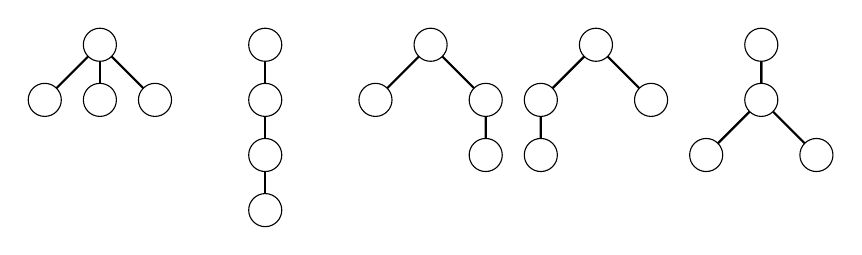
\begin{tikzpicture}[scale=0.7]
\path[draw,thick,-] (0,0) -- (-1,-1);
\path[draw,thick,-] (0,0) -- (0,-1);
\path[draw,thick,-] (0,0) -- (1,-1);
\draw[fill=white] (0,0) circle (0.3);
\draw[fill=white] (-1,-1) circle (0.3);
\draw[fill=white] (0,-1) circle (0.3);
\draw[fill=white] (1,-1) circle (0.3);

\path[draw,thick,-] (3,0) -- (3,-1) -- (3,-2) -- (3,-3);
\draw[fill=white] (3,0) circle (0.3);
\draw[fill=white] (3,-1) circle (0.3);
\draw[fill=white] (3,-2) circle (0.3);
\draw[fill=white] (3,-3) circle (0.3);

\path[draw,thick,-] (6+0,0) -- (6-1,-1);
\path[draw,thick,-] (6+0,0) -- (6+1,-1) -- (6+1,-2);
\draw[fill=white] (6+0,0) circle (0.3);
\draw[fill=white] (6-1,-1) circle (0.3);
\draw[fill=white] (6+1,-1) circle (0.3);
\draw[fill=white] (6+1,-2) circle (0.3);

\path[draw,thick,-] (9+0,0) -- (9+1,-1);
\path[draw,thick,-] (9+0,0) -- (9-1,-1) -- (9-1,-2);
\draw[fill=white] (9+0,0) circle (0.3);
\draw[fill=white] (9+1,-1) circle (0.3);
\draw[fill=white] (9-1,-1) circle (0.3);
\draw[fill=white] (9-1,-2) circle (0.3);

\path[draw,thick,-] (12+0,0) -- (12+0,-1) -- (12-1,-2);
\path[draw,thick,-] (12+0,0) -- (12+0,-1) -- (12+1,-2);
\draw[fill=white] (12+0,0) circle (0.3);
\draw[fill=white] (12+0,-1) circle (0.3);
\draw[fill=white] (12-1,-2) circle (0.3);
\draw[fill=white] (12+1,-2) circle (0.3);

\end{tikzpicture}
\end{center}

\section{Bao hàm - loại trừ}

\index{inclusion-exclusion}

\key{Bao hàm - loại trừ (Inclusion-exclusion)} là một kỹ thuật
có thể được sử dụng để đếm kích thước
của một hợp các tập hợp khi kích thước của
các giao được biết, và ngược lại.
Một ví dụ đơn giản của kỹ thuật này là công thức
\[ |A \cup B| = |A| + |B| - |A \cap B|,\]
trong đó $A$ và $B$ là các tập hợp và $|X|$
biểu thị kích thước của $X$.
Công thức có thể được minh họa như sau:

\begin{center}
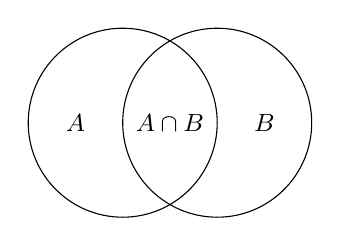
\begin{tikzpicture}[scale=0.8]

\draw (0,0) circle (1.5);
\draw (1.5,0) circle (1.5);

\node at (-0.75,0) {\small $A$};
\node at (2.25,0) {\small $B$};
\node at (0.75,0) {\small $A \cap B$};

\end{tikzpicture}
\end{center}

Mục tiêu của chúng ta là tính
kích thước của hợp $A \cup B$
tương ứng với diện tích của vùng
thuộc về ít nhất một vòng tròn.
Hình ảnh cho thấy chúng ta có thể tính
diện tích của $A \cup B$ bằng cách đầu tiên cộng
diện tích của $A$ và $B$ và sau đó trừ đi
diện tích của $A \cap B$.

Ý tưởng tương tự có thể được áp dụng khi số lượng
các tập hợp lớn hơn.
Khi có ba tập hợp, công thức bao hàm-loại trừ là
\[ |A \cup B \cup C| = |A| + |B| + |C| - |A \cap B|  - |A \cap C|  - |B \cap C| + |A \cap B \cap C| \]
và hình ảnh tương ứng là

\begin{center}
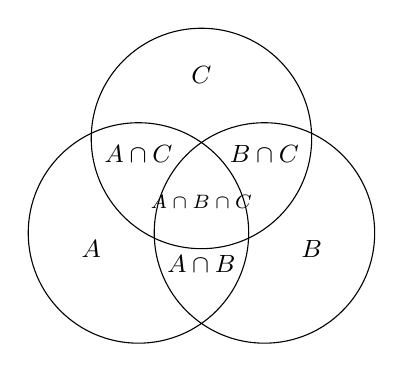
\begin{tikzpicture}[scale=0.8]

\draw (0,0) circle (1.75);
\draw (2,0) circle (1.75);
\draw (1,1.5) circle (1.75);

\node at (-0.75,-0.25) {\small $A$};
\node at (2.75,-0.25) {\small $B$};
\node at (1,2.5) {\small $C$};
\node at (1,-0.5) {\small $A \cap B$};
\node at (0,1.25) {\small $A \cap C$};
\node at (2,1.25) {\small $B \cap C$};
\node at (1,0.5) {\scriptsize $A \cap B \cap C$};

\end{tikzpicture}
\end{center}

Trong trường hợp tổng quát, kích thước của
hợp $X_1 \cup X_2 \cup \cdots \cup X_n$
có thể được tính bằng cách duyệt qua tất cả các
giao có thể có chứa một số các tập hợp $X_1,X_2,\ldots,X_n$.
Nếu giao chứa một số lẻ các tập hợp,
kích thước của nó được cộng vào câu trả lời,
và ngược lại, kích thước của nó được trừ khỏi câu trả lời.

Lưu ý rằng có các công thức tương tự
để tính
kích thước của một giao từ kích thước của
các hợp. Ví dụ,
\[ |A \cap B| = |A| + |B| - |A \cup B|\]
và
\[ |A \cap B \cap C| = |A| + |B| + |C| - |A \cup B|  - |A \cup C|  - |B \cup C| + |A \cup B \cup C| .\]

\subsubsection{Hoán vị mất chỗ}

\index{derangement}

Ví dụ, chúng ta hãy đếm số lượng các \key{hoán vị mất chỗ (derangements)}
của các phần tử $\{1,2,\ldots,n\}$, tức là, các hoán vị
trong đó không có phần tử nào ở vị trí ban đầu của nó.
Ví dụ, khi $n=3$, có
hai hoán vị mất chỗ: $(2,3,1)$ và $(3,1,2)$.

Một cách tiếp cận để giải quyết bài toán là sử dụng
bao hàm-loại trừ.
Gọi $X_k$ là tập hợp các hoán vị
chứa phần tử $k$ ở vị trí $k$.
Ví dụ, khi $n=3$, các tập hợp như sau:
\[
\begin{array}{lcl}
X_1 & = & \{(1,2,3),(1,3,2)\} \\
X_2 & = & \{(1,2,3),(3,2,1)\} \\
X_3 & = & \{(1,2,3),(2,1,3)\} \\
\end{array}
\]
Sử dụng các tập hợp này, số lượng các hoán vị mất chỗ bằng
\[ n! - |X_1 \cup X_2 \cup \cdots \cup X_n|, \]
vì vậy chỉ cần tính kích thước của hợp.
Sử dụng bao hàm-loại trừ, điều này quy về
việc tính kích thước của các giao có thể được
thực hiện một cách hiệu quả.
Ví dụ, khi $n=3$, kích thước của
$|X_1 \cup X_2 \cup X_3|$ là
\[
\begin{array}{lcl}
 & & |X_1| + |X_2| + |X_3| - |X_1 \cap X_2|  - |X_1 \cap X_3|  - |X_2 \cap X_3| + |X_1 \cap X_2 \cap X_3| \\
 & = & 2+2+2-1-1-1+1 \\
 & = & 4, \\
\end{array}
\]
vì vậy số lượng các giải pháp là $3!-4=2$.

Hóa ra bài toán cũng có thể được giải quyết
mà không cần sử dụng bao hàm-loại trừ.
Gọi $f(n)$ là số lượng các hoán vị mất chỗ
cho $\{1,2,\ldots,n\}$. Chúng ta có thể sử dụng
công thức đệ quy sau:

\begin{equation*}
    f(n) = \begin{cases}
               0               & n = 1\\
               1               & n = 2\\
               (n-1)(f(n-2) + f(n-1)) & n>2 \\
           \end{cases}
\end{equation*}

Công thức có thể được suy ra bằng cách xem xét
các khả năng cách phần tử 1 thay đổi
trong hoán vị mất chỗ.
Có $n-1$ cách để chọn một phần tử $x$
thay thế phần tử 1.
Trong mỗi lựa chọn như vậy, có hai tùy chọn:

\textit{Tùy chọn 1:} Chúng ta cũng thay thế phần tử $x$
bằng phần tử 1.
Sau đó, nhiệm vụ còn lại là xây dựng
một hoán vị mất chỗ của $n-2$ phần tử.

\textit{Tùy chọn 2:} Chúng ta thay thế phần tử $x$
bằng một phần tử khác 1.
Bây giờ chúng ta phải xây dựng một hoán vị mất chỗ
của $n-1$ phần tử, bởi vì chúng ta không thể thay thế
phần tử $x$ bằng phần tử 1, và tất cả các
phần tử khác phải được thay đổi.

\section{Bổ đề Burnside}

\index{Burnside's lemma}

\key{Bổ đề Burnside (Burnside's lemma)}
có thể được sử dụng để đếm
số lượng các kết hợp sao cho
chỉ có một đại diện được đếm
cho mỗi nhóm các kết hợp đối xứng.
Bổ đề Burnside phát biểu rằng số lượng các
kết hợp là
\[\sum_{k=1}^n \frac{c(k)}{n},\]
trong đó có $n$ cách để thay đổi
vị trí của một kết hợp,
và có $c(k)$ kết hợp
vẫn không thay đổi khi cách thứ $k$ được áp dụng.

Ví dụ, chúng ta hãy tính số lượng
các vòng cổ gồm $n$ hạt,
trong đó mỗi hạt có $m$ màu có thể.
Hai vòng cổ là đối xứng nếu chúng
giống nhau sau khi xoay chúng.
Ví dụ, vòng cổ
\begin{center}
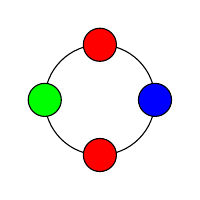
\begin{tikzpicture}[scale=0.7]
\draw[fill=white] (0,0) circle (1);
\draw[fill=red] (0,1) circle (0.3);
\draw[fill=blue] (1,0) circle (0.3);
\draw[fill=red] (0,-1) circle (0.3);
\draw[fill=green] (-1,0) circle (0.3);
\end{tikzpicture}
\end{center}
có các vòng cổ đối xứng sau:
\begin{center}
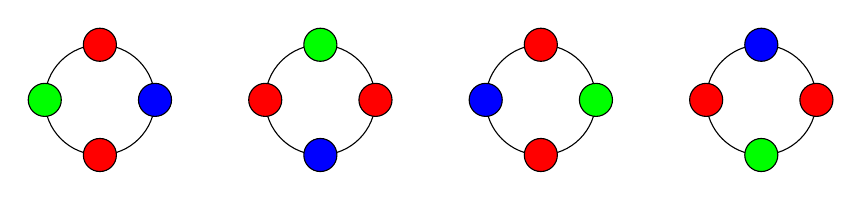
\begin{tikzpicture}[scale=0.7]
\draw[fill=white] (0,0) circle (1);
\draw[fill=red] (0,1) circle (0.3);
\draw[fill=blue] (1,0) circle (0.3);
\draw[fill=red] (0,-1) circle (0.3);
\draw[fill=green] (-1,0) circle (0.3);

\draw[fill=white] (4,0) circle (1);
\draw[fill=green] (4+0,1) circle (0.3);
\draw[fill=red] (4+1,0) circle (0.3);
\draw[fill=blue] (4+0,-1) circle (0.3);
\draw[fill=red] (4+-1,0) circle (0.3);

\draw[fill=white] (8,0) circle (1);
\draw[fill=red] (8+0,1) circle (0.3);
\draw[fill=green] (8+1,0) circle (0.3);
\draw[fill=red] (8+0,-1) circle (0.3);
\draw[fill=blue] (8+-1,0) circle (0.3);

\draw[fill=white] (12,0) circle (1);
\draw[fill=blue] (12+0,1) circle (0.3);
\draw[fill=red] (12+1,0) circle (0.3);
\draw[fill=green] (12+0,-1) circle (0.3);
\draw[fill=red] (12+-1,0) circle (0.3);
\end{tikzpicture}
\end{center}
Có $n$ cách để thay đổi vị trí
của một vòng cổ,
bởi vì chúng ta có thể xoay nó
$0,1,\ldots,n-1$ bước theo chiều kim đồng hồ.
Nếu số bước là 0,
tất cả $m^n$ vòng cổ vẫn giữ nguyên,
và nếu số bước là 1,
chỉ có $m$ vòng cổ trong đó mỗi
hạt có cùng một màu vẫn giữ nguyên.

Tổng quát hơn, khi số bước là $k$,
tổng cộng
\[m^{\textrm{gcd}(k,n)}\]
vòng cổ vẫn giữ nguyên,
trong đó $\textrm{gcd}(k,n)$ là ước chung lớn nhất
của $k$ và $n$.
Lý do cho điều này là các khối
hạt có kích thước $\textrm{gcd}(k,n)$
sẽ thay thế cho nhau.
Do đó, theo bổ đề Burnside,
số lượng các vòng cổ là
\[\sum_{i=0}^{n-1} \frac{m^{\textrm{gcd}(i,n)}}{n}. \]
Ví dụ, số lượng các vòng cổ có độ dài 4
với 3 màu là
\[\frac{3^4+3+3^2+3}{4} = 24. \]

\section{Công thức Cayley}

\index{Cayley's formula}

\key{Công thức Cayley (Cayley's formula)}
phát biểu rằng
có $n^{n-2}$ cây có nhãn
chứa $n$ nút.
Các nút được dán nhãn $1,2,\ldots,n$,
và hai cây là khác nhau
nếu cấu trúc của chúng hoặc
nhãn của chúng khác nhau.

\begin{samepage}
Ví dụ, khi $n=4$, số lượng các cây
có nhãn là $4^{4-2}=16$:

\begin{center}
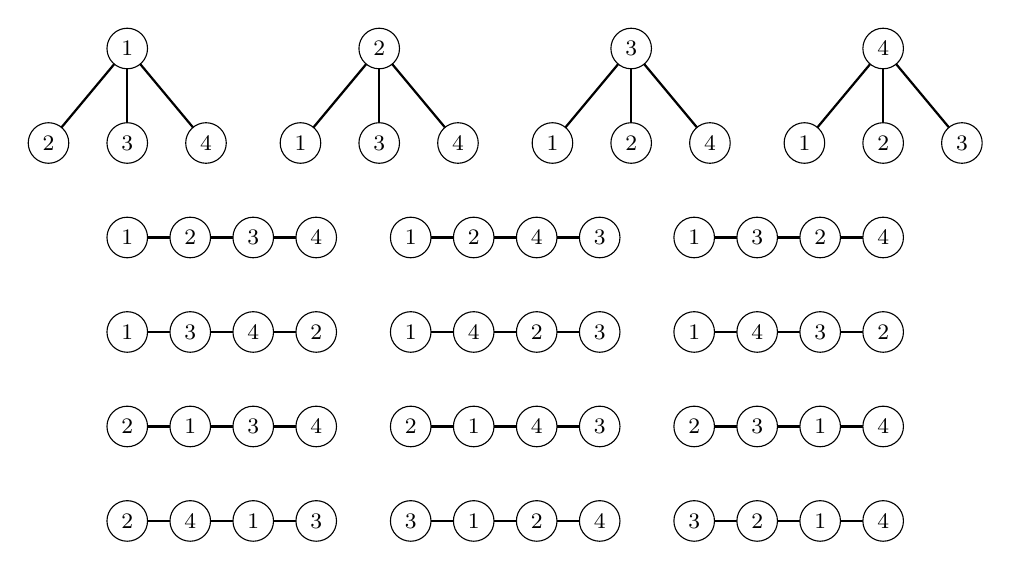
\begin{tikzpicture}[scale=0.8]
\footnotesize

\newcommand\puua[6]{
\path[draw,thick,-] (#1,#2) -- (#1-1.25,#2-1.5);
\path[draw,thick,-] (#1,#2) -- (#1,#2-1.5);
\path[draw,thick,-] (#1,#2) -- (#1+1.25,#2-1.5);
\node[draw, circle, fill=white] at (#1,#2) {#3};
\node[draw, circle, fill=white] at (#1-1.25,#2-1.5) {#4};
\node[draw, circle, fill=white] at (#1,#2-1.5) {#5};
\node[draw, circle, fill=white] at (#1+1.25,#2-1.5) {#6};
}
\newcommand\puub[6]{
\path[draw,thick,-] (#1,#2) -- (#1+1,#2);
\path[draw,thick,-] (#1+1,#2) -- (#1+2,#2);
\path[draw,thick,-] (#1+2,#2) -- (#1+3,#2);
\node[draw, circle, fill=white] at (#1,#2) {#3};
\node[draw, circle, fill=white] at (#1+1,#2) {#4};
\node[draw, circle, fill=white] at (#1+2,#2) {#5};
\node[draw, circle, fill=white] at (#1+3,#2) {#6};
}

\puua{0}{0}{1}{2}{3}{4}
\puua{4}{0}{2}{1}{3}{4}
\puua{8}{0}{3}{1}{2}{4}
\puua{12}{0}{4}{1}{2}{3}

\puub{0}{-3}{1}{2}{3}{4}
\puub{4.5}{-3}{1}{2}{4}{3}
\puub{9}{-3}{1}{3}{2}{4}
\puub{0}{-4.5}{1}{3}{4}{2}
\puub{4.5}{-4.5}{1}{4}{2}{3}
\puub{9}{-4.5}{1}{4}{3}{2}
\puub{0}{-6}{2}{1}{3}{4}
\puub{4.5}{-6}{2}{1}{4}{3}
\puub{9}{-6}{2}{3}{1}{4}
\puub{0}{-7.5}{2}{4}{1}{3}
\puub{4.5}{-7.5}{3}{1}{2}{4}
\puub{9}{-7.5}{3}{2}{1}{4}
\end{tikzpicture}
\end{center}
\end{samepage}

Tiếp theo chúng ta sẽ xem làm thế nào công thức Cayley có thể được
suy ra bằng cách sử dụng mã Prüfer.

\subsubsection{Mã Prüfer}

\index{Prüfer code}

Một \key{mã Prüfer (Prüfer code)}
là một dãy
$n-2$ số mô tả một cây có nhãn.
Mã được xây dựng bằng cách tuân theo một quy trình
loại bỏ $n-2$ lá khỏi cây.
Ở mỗi bước, lá có nhãn nhỏ nhất bị loại bỏ,
và nhãn của hàng xóm duy nhất của nó được thêm vào mã.

Ví dụ, chúng ta hãy tính mã Prüfer
của đồ thị sau:
\begin{center}
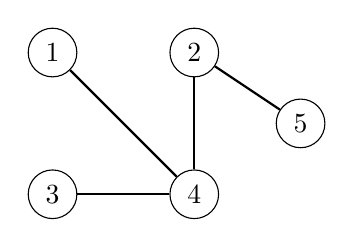
\begin{tikzpicture}[scale=0.9]
\node[draw, circle] (1) at (2,3) {$1$};
\node[draw, circle] (2) at (4,3) {$2$};
\node[draw, circle] (3) at (2,1) {$3$};
\node[draw, circle] (4) at (4,1) {$4$};
\node[draw, circle] (5) at (5.5,2) {$5$};

\path[draw,thick,-] (1) -- (4);
\path[draw,thick,-] (3) -- (4);
\path[draw,thick,-] (2) -- (4);
\path[draw,thick,-] (2) -- (5);
\end{tikzpicture}
\end{center}

Đầu tiên chúng ta loại bỏ nút 1 và thêm nút 4 vào mã:
\begin{center}
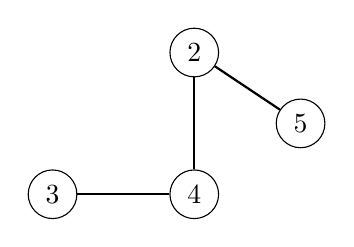
\begin{tikzpicture}[scale=0.9]
\node[draw, circle] (2) at (4,3) {$2$};
\node[draw, circle] (3) at (2,1) {$3$};
\node[draw, circle] (4) at (4,1) {$4$};
\node[draw, circle] (5) at (5.5,2) {$5$};

\path[draw,thick,-] (3) -- (4);
\path[draw,thick,-] (2) -- (4);
\path[draw,thick,-] (2) -- (5);
\end{tikzpicture}
\end{center}

Sau đó chúng ta loại bỏ nút 3 và thêm nút 4 vào mã:
\begin{center}
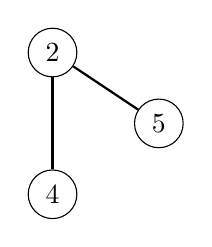
\begin{tikzpicture}[scale=0.9]
\node[draw, circle] (2) at (4,3) {$2$};
\node[draw, circle] (4) at (4,1) {$4$};
\node[draw, circle] (5) at (5.5,2) {$5$};

\path[draw,thick,-] (2) -- (4);
\path[draw,thick,-] (2) -- (5);
\end{tikzpicture}
\end{center}

Cuối cùng chúng ta loại bỏ nút 4 và thêm nút 2 vào mã:
\begin{center}
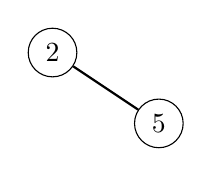
\begin{tikzpicture}[scale=0.9]
\node[draw, circle] (2) at (4,3) {$2$};
\node[draw, circle] (5) at (5.5,2) {$5$};

\path[draw,thick,-] (2) -- (5);
\end{tikzpicture}
\end{center}

Do đó, mã Prüfer của đồ thị là $[4,4,2]$.

Chúng ta có thể xây dựng một mã Prüfer cho bất kỳ cây nào,
và quan trọng hơn,
cây ban đầu có thể được tái tạo
từ một mã Prüfer.
Do đó, số lượng các cây có nhãn
gồm $n$ nút bằng
$n^{n-2}$, số lượng các mã Prüfer
có kích thước $n$.